%% The first command in your LaTeX source must be the \documentclass command.
%%
%% Options:
%% twocolumn : Two column layout. Do not use twocolumn for papers submitted to CEUR-WS!
%% hf: enable header and footer.
\documentclass[
% twocolumn,
% hf,
]{ceurart}

%%
%% One can fix some overfulls
\sloppy

%%
%% Minted listings support
%% Need pygment <http://pygments.org/> <http://pypi.python.org/pypi/Pygments>
\usepackage{listings}
%% auto break lines
\lstset{breaklines=true}

%% Necessario per la Figura 2 (topologia del testbed)
\usepackage{tikz}
\usepackage{adjustbox}
\usetikzlibrary{fit,backgrounds,positioning}

%%
%% end of the preamble, start of the body of the document source.
\begin{document}

%%
%% Rights management information.
%% CC-BY is default license.
\copyrightyear{2026}
\copyrightclause{Copyright for this paper by its authors.
  Use permitted under Creative Commons License Attribution 4.0
  International (CC BY 4.0).}

%%
%% This command is for the conference information
\conference{ITADATA2026: The 5$^{\text{th}}$ Italian Conference on Big Data and Data Science, November 10--12, 2026, Bari, Italy}

%% ---------------------------------------------------------------------
%% NOTE sui numeri [N] nel blocco titolo/autori (NON sono \footnote{}!):
%%
%% 1) \author[N,M]{...} -> N,M sono riferimenti alle AFFILIAZIONI:
%%    devono corrispondere esattamente ai numeri usati in \address[N]{...}.
%%    Un autore con piu' affiliazioni usa piu' numeri separati da virgola.
%%
%% 2) Le note (titolo/corresponding/generica) sono invece divise in un
%%    comando "mark" (mette il simbolo accanto al titolo/nome) e un
%%    comando "text" (il testo in fondo pagina), abbinati dallo stesso
%%    numero [N]. Qui [N] non e' un ID libero: seleziona un simbolo da
%%    una tabella FISSA per categoria:
%%      \tnotemark[N]/\tnotetext[N]  (sul titolo)      -> [1]=star, [2]=star star, ...
%%      \cormark[N]/\cortext[N]      (corresponding au) -> [1]=*, [2]=**, ...
%%      \fnmark[N]/\fntext[N]        (nota generica)    -> [1]=dagger, [2]=ddagger, [3]=paragraph, ...
%%    Piu' autori con lo stesso \fnmark[N] condividono lo stesso
%%    \fntext[N] (il testo va scritto una sola volta anche se si applica
%%    a piu' persone). Tutti i mark/text vanno messi prima di \maketitle.
%% ---------------------------------------------------------------------

%%
%% The "title" command
\title{Security Assurance for Modern Big Data APIs}

%\tnotemark[1]
%\tnotetext[1]{}

%%
%% The "author" command and its associated commands are used to define
%% the authors and their affiliations.
\author[1]{Enea Manzi}[%
  orcid=0009-0008-9490-1382,
  email=enea.manzi@studenti.unimi.it,
  url=https://eneamanzi.github.io/,
]
\cormark[1]
%\fnmark[1]

\author[1]{Marco Anisetti}[%
  orcid=0000-0002-5438-9467,
  email=marco.anisetti@unimi.it,
  url=https://anisetti.di.unimi.it/,
]
%\fnmark[1]

\address[1]{SESAR Lab, Dipartimento di Informatica "Giovanni Degli Antoni", Università degli Studi di Milano, Via Celoria 18, Milano, 20133, Italia}

%% Footnotes
\cortext[1]{Corresponding author.}
%\fntext[1]{These authors contributed equally.}

%%
%% The abstract is a short summary of the work to be presented in the
%% article.
\begin{abstract}
  %Modern Big Data systems increasingly deliver their value through pipelines composed of services distributed across microservice architectures, and every access to their data and processing capabilities crosses a REST API, typically exposed through a gateway.
  Modern Big Data systems often deliver value through distributed data pipelines and microservice-based architectures, with data and processing capabilities commonly exposed through APIs, frequently via an API gateway.
  %Assurance of such Big Data systems has so far been addressed mainly at the infrastructure and pipeline levels, while the interface level - where authentication, authorization, and data exposure are actually enforced - remains comparatively overlooked.

  Assurance of such Big Data systems has so far been addressed primarily on infrastructure and pipelines, with comparatively less attention to the interface layer where access control and data exposure are enforced.

  %Automated API testing compounds the gap: it has traditionally focused on functional correctness, and the few security-oriented tools operate at the syntactic level of requests and responses, unable to detect vulnerabilities tied to the target's semantic behavior.
  %Four of the top five categories in the OWASP API Security Top 10 (2023) belong to this class, and deriving evaluation criteria for them from security semantics remains one of the least explored challenges in the literature.

  Automated API testing has traditionally focused on functional correctness, while security testing remains limited. Existing approaches largely operate at the syntactic level of requests and responses, making them ineffective at detecting vulnerabilities that stem from semantic behavior, even though such vulnerabilities account for most of the top-ranked OWASP API security risks.

  %Existing solutions further trade portability off against depth, and non-deterministic execution undermines reproducibility.

  This work proposes a contract-driven approach to the security assurance of Big Data service APIs.
  Leveraging the target's OpenAPI specification, the framework generates syntactically valid probes and derives evaluation criteria from the semantics of the assessed controls, embedding them into deterministic test oracles organized into an eight-domain taxonomy that scales coverage with the privileges available during testing.
  The approach was validated on Forgejo 14.0.3 deployed behind Kong 3.9, instantiating the repository service through which Big Data pipelines are developed and delivered. Results show that the framework correctly classified all test cases, revealed a real discrepancy between the specification's declared requirements and the target's actual behavior, and produced identical outputs across independent runs.

  %Overall, this work contributes an implementation-agnostic eight-domain taxonomy for the security assurance of Big Data service interfaces, a systematic approach to the oracle problem grounded in security semantics, and a deterministic, DAG-based assessment engine ready for integration into automated delivery pipelines.
\end{abstract}

%%
%% Keywords. The author(s) should pick words that accurately describe
%% the work being presented. Separate the keywords with commas.
\begin{keywords}
  Big Data assurance \sep
  API security \sep
  REST \sep
  contract-driven testing \sep
  test oracles \sep
  reproducibility
\end{keywords}

%%
%% This command processes the author and affiliation and title
%% information and builds the first part of the formatted document.
\maketitle

% !TEX root = ../main.tex
%% ============================================================================
\section{Introduction}
\label{sec:intro}
%% ============================================================================

Modern Big Data systems deliver their value through pipelines composed of distributed services, (i.e., ingestion, storage, processing, serving) rather than through a single monolithic engine.
Trustworthiness in this setting cannot be a property of one layer alone: it must hold at the pipeline level, at the level of the ecosystem of services executing it, at the level of the data it governs, and at the interface level, and it must hold continuously, as pipelines evolve, rather than as a one-off certificate issued at deployment time.

Existing work on Big Data assurance addresses the first two levels. Anisetti et al. propose an assurance process for Big Data pipelines and their underlying ecosystem~\cite{anisettiAssuranceProcessBig2023}; Ardagna et al. address the same problem through service-level agreements~\cite{ardagnaBigDataAssurance2023}; continuous verification across the pipeline life cycle has been framed as a DevSecOps activity~\cite{anisettiDevSecOpsbasedAssuranceProcess2022}; and access control has been enforced at data-ingestion time, an approach recently extended into an attribute-based data engine~\cite{anisettiDynamicScalableEnforcement2021,polimenoBalancingProtectionQuality2025}.
Across this body of work, the interface level is the least covered.

Yet the interface is where enforcement actually happens. Every access to a Big Data pipeline and to the data it processes crosses an API, typically exposed through a gateway that concentrates authentication, authorization, and rate limiting; a guarantee proven at the pipeline level does not propagate end-to-end if the API exposing that pipeline is permeable.

Automated API testing does not close this gap. Golmohammadi et al. presents a systematic review of 92 contributions shows that only 8 address security testing explicitly~\cite{golmohammadiTestingRESTfulAPIs2023}; and even where security is the explicit target, building the evaluation criteria that decide whether an observed behaviour violates a security guarantee remains the least solved problem in test automation~\cite{barrOracleProblemSoftware2015}.

In this paper we propose a contract-driven approach to the security assurance of Big Data service APIs, in which the target's OpenAPI specification governs the construction of syntactically valid probes and the evaluation criterion of each test is derived from the domain knowledge of the security control being exercised, rather than from the syntax of the request or response alone. The approach is organised around three research questions:

\begin{itemize}
  \item \textbf{RQ1}: Can security guarantees of an API be verified beyond syntactic conformance, using criteria derived from the semantics of the security controls themselves?
  \item \textbf{RQ2}: Can such verification be made deterministic and reproducible across independent executions, so that it can be embedded in a continuous release cycle?
  \item \textbf{RQ3}: Does the resulting approach correctly distinguish enforced from bypassed guarantees on a real target, including anomalies not anticipated in advance?
\end{itemize}

The contributions of this paper are threefold: (i) an implementation-agnostic eight-domain taxonomy for the security assurance of service APIs, with privilege-aware coverage; (ii) a systematic use of specified oracles in API security testing, with evaluation criteria derived from the semantics of each control; and (iii) a deterministic, DAG-based assessment engine whose output is reproducible and machine-actionable, together with its empirical validation.

The remainder of the paper is organised as follows. Section~\ref{sec:related} discusses related work. Section~\ref{sec:scenario} details the reference scenario. Section~\ref{sec:method} presents the contract-driven approach. Section~\ref{sec:eval} reports the experimental evaluation. Section~\ref{sec:conclusions} draws our conclusions and outlines future work.




% !TEX root = ../main.tex
%% ============================================================================
\section{Related Work and Gaps}
\label{sec:related}
%% ============================================================================

%Two lines of work meet in this paper: assurance of Big Data systems, and automated testing of REST APIs.

%\paragraph{Assurance of Big Data systems.}
The trustworthiness of Big Data computations has been addressed as a property of the pipeline, of the ecosystem of services executing it, and of the data it governs.
Anisetti et al. propose an assurance process that jointly evaluates a Big Data pipeline and its underlying ecosystem, annotating pipeline templates with non-functional requirements and computing an aggregate trustworthiness confidence level, validated on a Big-Data-Analytics-as-a-Service platform~\cite{anisettiAssuranceProcessBig2023}.
Ardagna et al. address the same problem through service-level agreements, negotiating and monitoring contractual guarantees, such as data integrity and availability, between the parties of a Big-Data-Analytics-as-a-Service deployment~\cite{ardagnaBigDataAssurance2023}.
Continuous verification across the pipeline life cycle has been framed as a DevSecOps activity, embedding assurance checks for non-functional requirements at every stage from planning to operation~\cite{anisettiDevSecOpsbasedAssuranceProcess2022}.
At the data governance level, access control has been enforced at ingestion time through data annotations and secure transformations~\cite{anisettiDynamicScalableEnforcement2021}, an approach recently extended into an attribute-based data engine that balances data protection against analytics quality~\cite{polimenoBalancingProtectionQuality2025}.
These contributions target the pipeline, the ecosystem executing it, and the data governed within it; none addresses the REST interface through which every access to that pipeline and that data actually takes place, an assumption on which their own guarantees implicitly rely.
That assumption is what we make verifiable.

%\paragraph{Automated testing of REST APIs.}
%A systematic review of 92 contributions published between 2009 and 2022~\cite{golmohammadiTestingRESTfulAPIs2023} shows that the field concentrated on system testing, understood as verifying that the API responds correctly and respects the declared formats: 72 of the 92 papers fall in this category.
%Security testing is addressed explicitly by 8 papers and listed as an open challenge by 10 more.
Considering the automated testing of REST APIs, it still in its infancy and is considered as an open challenge. Du et al. identified that just 2--5\% of the detected HTTP~500 faults correspond to actual security vulnerabilities~\cite{duVulnerabilityorientedTestingRESTful2024}.

The contract-driven line of research is focused on replacing syntactic heuristics with knowledge of the formal specification.
RESTler infers producer, consumer dependencies from the OpenAPI specification, and generates stateful request sequences. Its oracle is the HTTP~500 status code, which the authors acknowledge cannot reach vulnerabilities that do not manifest through status codes~\cite{atlidakisRESTlerStatefulREST2019a}.
Atlidakis et al. extend it with four formal security rules and active property checkers~\cite{atlidakisCheckingSecurityProperties2020}; NAUTILUS orients the paradigm towards injection-class vulnerabilities requiring ordered operation sequences~\cite{dengNAUTILUSAutomatedRESTful2023}; Schemathesis derives a structured set of conformance properties from the specification and from RFC~7231~\cite{schemathesisDerivingSemanticsawareFuzzers2022}.
A distinct direction automates the construction of the oracle itself, dynamically from observed request/response pairs~\cite{alonsoAGORAAutomatedGeneration2023, alonsoAgora+TestOracleGeneration2025} or statically from the specification~\cite{alonsoSATORIStaticTest2025}; both operate in the domain of functional conformance.
Closest to our objective, Sahin et al. propose nine automated oracles for authorization, authentication, and injection faults, applied as a post-processing phase over an existing fuzzer~\cite{sahinEnhancingRESTAPI2026}; the approach is confined to the application layer and does not cover the configuration of the gateway that fronts the service.
Table~\ref{tab:related} summarises how these approaches use the specification and where their oracle stops.

\begin{table}
  \small
  \caption{What each contract-driven approach checks, and where its oracle stops.}
  \label{tab:related}
  \begin{tabular}{l p{0.28\textwidth} p{0.30\textwidth}}
    \toprule
    \textbf{Approach}                                                                           & \textbf{What it checks}                                                             & \textbf{Oracle boundary}              \\
    \midrule
    RESTler~\cite{atlidakisRESTlerStatefulREST2019a}                                            & Server crashes                                                                      & Only HTTP~500; no semantic check      \\
    Atlidakis et al.~\cite{atlidakisCheckingSecurityProperties2020}                             & Use-after-free, resource leak, hierarchy and namespace violations                   & Fixed rules, no config.\ adaptability \\
    NAUTILUS~\cite{dengNAUTILUSAutomatedRESTful2023}                                            & SQL/command injection, XSS, privilege escalation                                    & Injection-focused only                \\
    Schemathesis~\cite{schemathesisDerivingSemanticsawareFuzzers2022}                           & Schema conformance, undeclared status codes                                         & Structural, no security check         \\
    AGORA/AGORA+~\cite{alonsoAGORAAutomatedGeneration2023,alonsoAgora+TestOracleGeneration2025} & Functional conformance (mined invariants)                                           & Contract only, no security            \\
    SATORI~\cite{alonsoSATORIStaticTest2025}                                                    & Functional conformance (static, via LLM)                                            & Contract only, no security            \\
    Sahin et al.~\cite{sahinEnhancingRESTAPI2026}                                               & Authorization/authentication violations, exposed stack traces, undeclared endpoints & Application layer only, no gateway    \\
    \bottomrule
  \end{tabular}
\end{table}

%The approaches above already expose two of the four gaps that motivate this work.
Given the current related work the following gaps emerge:
Syntactic blindness (\textbf{G1}): what each tool checks, summarised in Table~\ref{tab:related}, is either a status code, a structural property of the response, or a fault class mined or authored independently of the target's security semantics; none of them evaluates whether a syntactically valid request violates the access rules the system is supposed to enforce.
The absence of evaluation criteria for security guarantees (\textbf{G2}): deciding automatically whether an observed behaviour violates such a guarantee requires a criterion that the interface specification alone cannot supply, since it depends on the domain knowledge of the control being exercised.
Barr et al. survey this as the oracle problem, and identify the automated construction of such criteria as the bottleneck of test automation~\cite{barrOracleProblemSoftware2015}. AGORA/AGORA+ and SATORI build oracles explicitly, but mine or infer them from observed traffic or from the contract alone, targeting functional conformance rather than security semantics. Sahin et al. come closer, authoring nine fixed oracles for authorization, authentication, and injection faults, but the result is a closed set confined to the application layer, not a methodology that extends to new domains or to the gateway's own configuration \cite{sahinEnhancingRESTAPI2026}.

\revMin{Lack of Security Contract Validation in Cross-Target Tools (\textbf{G3}): Portable tools can leverage specifications to generate syntactically valid requests across different targets, but they do not verify whether the corresponding responses comply with the security properties declared in those specifications. As a result, portability is achieved at the expense of security-aware semantic validation.}
\revFix{Specification-driven approaches achieve their structural coverage by operating on the syntax of the OpenAPI document, and this same reliance leaves them unable to capture dynamic authorization rules or to detect violations that require understanding the security policies governing resource access}~\cite{abinayaSecurityTestingRESTful2027}.
% Dal paper abinayaSecurityTestingRESTful2027: 
% Although specification-based approaches provide strong structural coverage and automated input generation, they remain constrained by incomplete specifications and limited semantic understanding. Consequently, they often fail to detect undocumented runtime behaviors, authorization flaws, and complex business logic vulnerabilities.
% Dal papaer: Challenges: Specification-driven fuzzing techniques depend on static OAS documents and focus on the syntactic behavior of APIs [37, 57,58]. These methods cannot capture dynamic authorization rules, like role-based restrictions, token reuse, or session expiration. Functional correctness can be validated through status codes and schema vali dation [58,71]. However, detecting authorization violations requires understanding security policies that govern resource access [94].

\revMin{Absence of Deterministic Execution for Continuous Verification (\textbf{G4}): Existing approaches lack deterministic execution, leading to variations in results across successive runs. This prevents reliable comparison of outcomes over time and hinders the integration of automated verification into continuous release and deployment pipelines.}
\revFix{Non-deterministic, or flaky, test outcomes undermine continuous integration by causing builds to fail independently of any genuine fault, an effect observed for automatically generated test suites as much as for developer-written ones}~\cite{parrySurveyFlakyTests2021}. \revFix{An industrial account of API test automation for continuous delivery reports the same symptom directly, noting that automated test suites tend to pass and fail unpredictably, so that even a successful run does not provide reliable confidence to stakeholders}~\cite{bennettPracticalMethodAPI2021}.
% Dal paper parrySurveyFlakyTests2021:
% Tests that fail inconsistently, without changes to the code under test, are described as flaky. Flaky tests do not give a clear indication of the presence of software bugs and thus limit the reliability of the test suites that contain them. A recent survey of software developers found that 59% claimed to deal with flaky tests on a monthly, weekly, or daily basis.
% In a continuous integration system, when a developer has been working on their own branch and goes to merge their changes, their code is remotely built and a test suite run is triggered to ensure their changes have not introduced bugs. Should any tests fail, their changes will be rejected. Naturally, given the association between flaky tests and false alarm failures , flaky tests can limit the efficiency of the continuous integration process by incorrectly causing builds to fail
% [Sez. 4.3.3] These findings demonstrate that automated tools, as well as developers, are also capable of producing flaky tests, threatening the overall reliability of automatically generated test suites.
% [Sez. 4.3.3] regression test suites are useful in as far as they capture the behavior of a program at a given point in time and are used to identify if a recent code change has any unintended effects. If a regression test suite contains flaky tests, then it does not accurately reflect the behavior of the program and is thus less informative for developers.

% Dal paper bennettPracticalMethodAPI2021:
% The first problem is that execution of tests tends to fail and pass in seemingly nondeterministic ways (tests are flaky).
% The automated tests failed and passed in seemingly nondeterministic ways - the tests were flaky.
% So even a successful test run did not provide clear confidence for relevant stakeholders.



% !TEX root = ../main.tex
%% ============================================================================
\section{Reference Scenario}
\label{sec:scenario}
%% ============================================================================

%We consider the development and delivery of Big Data pipelines.
%In this scenario, pipeline code, deployment descriptors, build artefacts, and the webhooks that trigger orchestration are managed by a \emph{repository service} that data engineers from different tenants use to upload, version, and activate their pipelines.
%The service is exposed as a REST API behind an API gateway, which concentrates authentication, authorization, and rate limiting on a single, inspectable configuration plane and constitutes the boundary between clients and internal services~\cite{roseZeroTrustArchitecture2020}.

%This service belongs to the trust perimeter of the pipelines it hosts, and its API is where that perimeter is enforced.
%A broken object-level authorization check on that API exposes the code and configuration of another tenant's pipeline; an unverified webhook lets an unauthorised party trigger a pipeline execution; an endpoint that responds without credentials while the published specification declares it protected invalidates the assumptions that consumers of that service legitimately make.
%None of these failures is visible to an assessment conducted one level below, on the pipeline or on the infrastructure: the requests that realise them are syntactically impeccable, and four of the top five categories of the OWASP API Security Top~10 belong to this class~\cite{OWASPTop10}.

%NIST SP~800-228 formalises the same limit for cloud-native APIs, observing that payload-level defences cannot operate at the semantic level of the interface, and prescribing a formal specification with declared request and response schemas as a precondition for any automated verification~\cite{chandramouliGuidelinesAPIProtection2026}.

%The assurance problem we address is therefore the following: given a service of this kind, described by an OpenAPI specification and exposed through a gateway, decide automatically and reproducibly whether the security guarantees its contract declares are actually enforced.

We consider a Big Data platform in which data scientist design, deploy, and operate data-processing pipelines on behalf of multiple tenants. The lifecycle of these pipelines includes source-code development, artefact generation, deployment configuration, execution triggering, and version management. To support these activities, the platform exposes a \emph{repository service} that allows for storing, versioning, publishing, and activating pipelines. Pipeline code, deployment descriptors, build artefacts, and the orchestration are all managed through this service.

The repository service is exposed through a REST API protected by an API gateway. The gateway centralizes authentication, authorization, and rate-limiting policies, providing a single and inspectable control point where all the external requests are enforced~\cite{roseZeroTrustArchitecture2020}. This sevice API constitutes the main trust boundary between clients and the internal components responsible for the big data pipeline storage, deployment, and execution. The correctness of its interface-level security controls directly impacts the security of the entire platform. For example, a broken object-level authorization mechanism may allow one tenant to access the source code or configuration of another tenant's pipeline. Similarly, an improperly protected hook endpoint may enable unauthorized triggering of pipeline executions, while an endpoint that accepts requests without authentication despite being specified as protected violates the security assumptions made by service consumers.
We note that these vulnerabilities that emerge at the semantic level of the API contract, are largelly not addressed by traditional assessments focused mostly on the lowest layers involving pipeline code, runtime infrastructure, or network configuration.
Recent guidance, such as NIST SP 800-228, highlights the same limitation for cloud-native APIs, noting that payload-level and infrastructure-level protections cannot reason about the semantic correctness of API behavior~\cite{chandramouliGuidelinesAPIProtection2026}.

In our scenario we assume that the API of the repository service is accompanied by a formal machine-readable specification (i.e., OpenAPI) that explicitly defines operations, request and response schemas, and security requirements.

In this context the assurance problem addressed in this paper is the following. Given a Big Data repository service described by an OpenAPI specification and exposed through an API gateway, determine automatically whether the security guarantees declared in its API contract are actually enforced by the deployed implementation.



%% ============================================================================
\section{Contract-Driven API Assurance}
\label{sec:method}
%% ============================================================================

\subsection{Design Principles}

Four principles govern the approach.

\emph{Application agnosticism.} All knowledge of the target is derived at runtime from two sources only: the OpenAPI specification and a configuration file that supplies deployment-specific values, such as concrete values for parameterised paths and credentials for each configured role.
No reference to any specific system is hardcoded, so the approach applies to any documented REST API without modifying code and without access to the source of the target.

\emph{Contract-driven probing.} The specification is the contractual foundation of the whole process.
It governs the construction of requests that respect the declared types, formats, and constraints, so that probes are not rejected by the input validation layer before reaching the application logic; it delimits the assessment surface to the documented endpoints, which makes any endpoint responding outside that set a shadow API by definition; and it supplies the primary structural criterion against which responses are evaluated.
Using a formal specification to build valid requests and using it to judge responses are distinct capabilities, and existing approaches largely stop at the first~\cite{atlidakisRESTlerStatefulREST2019a}.

\emph{Configuration as the single source of variation.} Every operational parameter -- timeouts, thresholds, priority filters, output paths -- resides in the configuration file; credentials reside in a separate, non-versioned file and are interpolated before parsing.
If behaviour changes between two executions, it is because the configuration changed.

\emph{Deterministic reproducibility.} The same target, in the same configuration, must produce identical results at every execution.
This is the property that turns an assessment from a single observation into a comparable measurement, and it is a precondition for the empirical claims of Section~\ref{sec:eval}.

\subsection{An Eight-Domain Assurance Taxonomy}

Security guarantees are organised in eight domains, reported in Table~\ref{tab:domains}, aligned with the risk categories and runtime controls that NIST SP~800-228 identifies for cloud-native APIs~\cite{chandramouliGuidelinesAPIProtection2026}.
The taxonomy is independent of any implementation: it partitions the security surface of an API exposed through a gateway into semantically distinct categories, each with its own evaluation criteria and priorities, and it is applicable to any structured assessment regardless of the tooling employed.

\begin{table}
  \caption{The eight assurance domains.}
  \label{tab:domains}
  %% SOURCE: Tesi/assets/tables/3-domini.tex — translate, shorten the scope column.
  \begin{tabular}{p{0.08\textwidth} p{0.22\textwidth} p{0.58\textwidth}}
    \toprule
    \textbf{Domain} & \textbf{Title}                    & \textbf{Scope of verification}                                                                    \\
    \midrule
    D0              & API Discovery                     & Inventory of exposed endpoints; detection of shadow APIs not documented in the specification.     \\
    D1              & Identity \& Authentication        & Caller recognition mechanisms; robustness of credential transport; JWT life cycle and revocation. \\
    D2              & Authorization                     & Access control logic; horizontal and vertical segregation defects (RBAC, BOLA).                   \\
    D3              & Data Integrity                    & Structural coherence of payloads; implementation of cryptographic signatures (HMAC).              \\
    D4              & Availability \& Resilience        & Defences against resource exhaustion; audit of circuit breakers and rate-limiting thresholds.     \\
    D5              & Observability                     & Quality and timeliness of the telemetry the system produces.                                      \\
    D6              & Configuration \& Hardening        & Hardening of the gateway configuration; routing policies; HTTP security headers.                  \\
    D7              & Business Logic \& Sensitive Flows & Complex semantic flaws: process constraint evasion, SSRF, race conditions on critical operations. \\
    \bottomrule
  \end{tabular}
\end{table}

The first three domains form a chain of preconditions.
Verifying authorization (D2) without having established that authentication works (D1) collects evidence about a system whose behaviour under compromised authentication is unknown, and verifying authentication without knowing the attack surface (D0) leaves that evidence incomplete.
Domains D3--D7 belong to distinct semantic families with no mutual ordering constraint.
Domain D5 (Observability) is architecturally provisioned but carries no active tests in the implementation evaluated here; its numbering is reserved to preserve the coherence of the sequence.

\subsection{Specified Oracles for Security Guarantees}
\label{sec:oracles}

Generating inputs automatically is a largely solved problem; deciding whether the observed behaviour is correct is the structural bottleneck of test automation.
Barr et al. formalise a test oracle as a partial function $D: T_A \to \mathbb{B}$ mapping a sequence of activities to a verdict, and distribute automation techniques over four categories: \emph{specified} oracles, derived from formal specifications; \emph{derived} oracles, inferred from artefacts such as previous executions; \emph{implicit} oracles, covering universal anomalies such as crashes; and \emph{no-oracle} strategies~\cite{barrOracleProblemSoftware2015}.

We adopt \emph{specified oracles} defined a~priori for every individual test and derived from the domain knowledge of the security control being exercised.
The methodological procedure is uniform. The class of verification is analysed, the relevant failure conditions are identified, and the criterion is encoded in the logic of the corresponding test.
What varies is the source from which the criterion is drawn, and that source is determined by the control, not by the target.
Table~\ref{tab:oracles} illustrates this mapping with representative tests drawn from across the eight domains; the same procedure applies uniformly to every test in the suite.

\begin{table}
  \caption{Sources of the evaluation criterion, by class of guarantee.}
  \label{tab:oracles}
  \begin{tabular}{p{0.20\textwidth} p{0.33\textwidth} p{0.39\textwidth}}
    \toprule
    \textbf{Class of guarantee}     & \textbf{Source of the criterion}                                             & \textbf{Verdict rule (example)}                                                                              \\
    \midrule
    Attack-surface conformance      & Set difference between responding and documented endpoints                   & an endpoint that responds without being declared is a shadow API                                             \\
    Response structural conformance & Contractual schema declared in the specification                             & a field present in the response but absent from the declared schema is a violation                           \\
    Protocol-level requirements     & Published technical standards                                                & a deprecated endpoint returning neither \texttt{410 Gone} nor a \texttt{Sunset} header is a violation        \\
    Authentication enforcement      & \texttt{security} markers of the specification, plus credential-less probing & a \texttt{2xx} response to an unauthenticated request on an endpoint declared as protected is a bypass       \\
    Authorization                   & Comparison of responses obtained with credentials of distinct roles          & a resource of one role readable with the credentials of another is a violation                               \\
    Infrastructural guarantees      & Direct inspection of the gateway configuration plane                         & the absence of a required security header (e.g. HSTS) in the gateway's declared configuration is a violation \\
    \bottomrule
  \end{tabular}
\end{table}

Two consequences follow, one operational and one epistemic.

Operationally, a fixed criterion makes the verdict invariant: the same system, interrogated in the same configuration, always yields the same outcome.
This is what makes assessments comparable across successive executions and grounds the reproducibility claim empirically rather than by assertion.
To keep that invariance from producing false positives, every HTTP probe is classified under a three-valued encoding rather than a binary one: \textsc{enforced}, the control works; \textsc{bypassed}, the control is absent or misconfigured; and \textsc{inconclusive}, the response cannot be interpreted with sufficient certainty to justify a finding.
A \texttt{404} on a parameterised path, for instance, may mean that the gateway rejected the request, that the path does not exist for the value used in the probe, or that the endpoint is genuinely unprotected but the path was wrong; treating it uniformly as a failure would make the assessment unusable.

Epistemically, the correctness of the verdicts is conditional on the correctness of the contract taken as reference.
A specification that is incomplete reduces the observable surface without the process being able to detect it; a specification that is contractually wrong produces evaluations grounded in a wrong oracle.
We return to this limit in Section~\ref{sec:threats}, and Section~\ref{sec:discrepancy} reports a concrete instance of it.

\subsection{Privilege-Aware Coverage}

Some guarantees are physically unreachable without a specific level of privilege, and that inaccessibility -- not a retroactive label -- is what determines the visibility level of a test.
Perimeter controls that the gateway applies to any interlocutor presuppose no knowledge of the internal infrastructure, and executing them without credentials is the only way to obtain evidence uncontaminated by implicit privileges: these are \texttt{BLACK\_BOX} tests, requiring network access alone.
An RBAC authorization control requires the system to be in an authenticated state under at least two distinct role identities, because the defect emerges only from comparing what two identities obtain on the same resource: these are \texttt{GREY\_BOX} tests.
Guarantees that reside in the static configuration of the gateway are verifiable only by direct inspection of its control plane, since no response on the exposed endpoints carries that information: these are \texttt{WHITE\_BOX} tests.

Each test declares its strategy as fixed metadata, so assessment depth adapts to the preconditions actually available in a given organisational context without requiring different versions of the tool: the variation lives in the configuration file, not in a mode switch.

\subsection{Deterministic Assessment Engine}

The assessment unfolds in seven sequential phases with differentiated error semantics.
The first four are blocking: initialisation, which validates the configuration and resolves credentials; retrieval and validation of the OpenAPI specification, which builds the map of exposed endpoints; construction of the execution contexts, which assembles the immutable target knowledge and the mutable runtime state; and discovery and scheduling of the tests, which resolves declared dependencies into an execution order.
A failure in any of these four halts the process before any test runs.
The last three are non-blocking: execution, which runs each test in the scheduled order; teardown, which reverses the resources any test created in last-in-first-out order; and reporting, which aggregates outcomes into machine-readable artefacts.
An error in any of them is isolated as a structured result, and the process continues.

Tests declare their dependencies explicitly, and a scheduler resolves them topologically into batches, each grouping the tests whose prerequisites were satisfied in the preceding batches.
This structure does more than establish an order: its purpose is semantic correctness.
A test that verifies token revocation presupposes that authentication has already been confirmed and a valid token acquired, and without a declared dependency the test's outcome would depend on execution order rather than on the target's actual behaviour.
Cycles in the declared dependencies are detected statically, before any test runs, and block the assessment before it starts.
A separate stall guard protects against a rarer failure mode: even in an acyclic graph, the scheduler can reach a state where tests remain but none of them is ready; when this happens, the guard reports the exact set of tests that could never be scheduled, rather than failing with a generic error.

Determinism is obtained by the conjunction of four mechanisms: a configuration that fixes every decisional parameter, so that the process has no endogenous sources of variation; a topological resolution that always produces the same batch sequence; a lexicographic ordering of the tests within each batch, which is the only source of a total order among tests that are ready at the same level; and the fixed oracles of Section~\ref{sec:oracles}.
Timestamps and record identifiers vary by nature; what must be invariant are the aggregate counters, the per-test verdicts, and the distribution of findings across domains.

Finally, the process terminates with one of four semantically distinct exit codes: \texttt{0} when every active test passed or was skipped; \texttt{1} when at least one violation was detected; \texttt{2} when no violation was detected but at least one test produced an internal error; and \texttt{10} on an infrastructural error that prevented execution.
Because the codes are semantically distinct, a CI/CD pipeline can route on the exit code alone, without parsing logs: a violation (\texttt{1}) calls for analysing and correcting the target, while an infrastructural error (\texttt{10}) calls for diagnosing the assessment's own deployment.


% !TEX root = ../main.tex
%% ============================================================================
\section{Experimental Evaluation}
\label{sec:eval}
%% ============================================================================

\subsection{Testbed}

% OLD
% \revTtwo{We use Forgejo~14.0.3} \cite{forgejoContributors2026} \revTtwo{as the target, instantiating the repository service of the reference scenario of} Section~\ref{sec:scenario}.
%\revTtwo{Forgejo is a self-hosted Git service exposing repositories, users, tokens, and webhooks through a REST API documented by a natively generated OpenAPI specification, with real authentication, two distinct privilege levels, and parameterised endpoints with resolvable path values.}

We use Forgejo~14.0.3 \cite{forgejoContributors2026} as the target, because it exposes the interface-layer properties that Section~\ref{sec:scenario} requires, none of which is specific to Forgejo -- they are common to any service exposed this way.
Concretely, Forgejo is a self-hosted Git service exposing repositories, users, tokens, and webhooks through a REST API documented by a natively generated OpenAPI specification, with real authentication, two distinct privilege levels, and parameterised endpoints with resolvable path values.

Forgejo is exposed through Kong~3.9~\cite{kongGateway2026} in DB-less mode, with PostgreSQL~15-alpine as Forgejo's persistence backend; an ephemeral container provisions three accounts at first start -- an administrator and two ordinary users -- and terminates.
All services run in a dedicated Docker network declared in a single Compose file, on a development host, without dedicated hardware.
Figure~\ref{fig:testbed} shows the topology.
Kong exposes three ports: plain HTTP for the redirect test, HTTPS with a locally generated self-signed certificate as the primary endpoint, and the Admin API supplying configuration data to the \texttt{WHITE\_BOX} tests.
DB-less mode matters for validation: the configuration lives entirely in a version-controlled file mounted read-only and cannot be altered at runtime, which guarantees that the gateway state is identical at every start.

Because the implementation contains no reference to Forgejo, changing target means updating the configuration file -- gateway URL, specification path, path seeds, credentials -- not modifying code.
This is the concrete demonstration of the application agnosticism claimed in Section~\ref{sec:method}, and it is why the same suite applies unchanged to any other service exhibiting the interface-layer properties of Section~\ref{sec:scenario}.

\begin{figure}[t]
  \centering
  \begin{adjustbox}{max width=\columnwidth}
    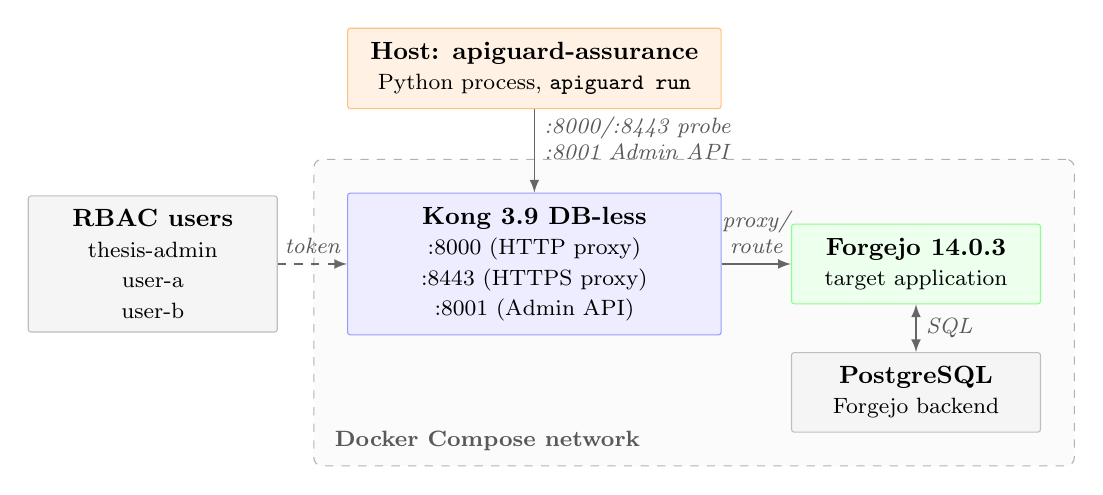
\begin{tikzpicture}[
        node distance=4ex and 2.5em,
        cls/.style={draw, rounded corners=1pt, inner sep=5pt, align=center, font=\small, minimum height=3.5ex},
        host/.style={cls, fill=orange!10, draw=orange!50, minimum width=13.5em},
        infra/.style={cls, fill=blue!7, draw=blue!40, minimum width=13.5em},
        app/.style={cls, fill=green!7, draw=green!45, minimum width=9em},
        backend/.style={cls, fill=gray!8, draw=gray!50, minimum width=9em},
        users/.style={cls, fill=gray!8, draw=gray!50, minimum width=9em},
        group/.style={draw=gray!60, fill=gray!3, dashed, inner sep=12pt, rounded corners=3pt},
        arr/.style={-latex, semithick, gray!80!black},
        darr/.style={-latex, semithick, dashed, gray!80!black},
        barr/.style={latex-latex, semithick, gray!80!black},
      ]

      \node[host] (host) {\textbf{Host: apiguard-assurance}\\{\footnotesize Python process, \texttt{apiguard run}}};

      \node[infra, below=7ex of host] (kong) {\textbf{Kong~3.9 DB-less}\\{\footnotesize :8000 (HTTP proxy)}\\{\footnotesize :8443 (HTTPS proxy)}\\{\footnotesize :8001 (Admin API)}};

      \node[app, right=2.5em of kong] (forgejo) {\textbf{Forgejo~14.0.3}\\{\footnotesize target application}};

      \node[users, left=2.5em of kong] (rbac) {\textbf{RBAC users}\\{\footnotesize thesis-admin}\\{\footnotesize user-a}\\{\footnotesize user-b}};

      \node[backend, below=4ex of forgejo] (pg) {\textbf{PostgreSQL}\\{\footnotesize Forgejo backend}};

      \begin{scope}[on background layer]
        \node[group, fit=(kong)(forgejo)(pg)] (compose) {};
      \end{scope}
      \node[font=\footnotesize\bfseries, text=gray!70!black, anchor=south west, xshift=1ex, yshift=0.5ex] at (compose.south west) {Docker Compose network};

      \draw[arr] (host.south) -- node[pos=0.35, right, align=left, font=\footnotesize\itshape, text=gray!70!black] {:8000/:8443 probe \\ :8001 Admin API} (kong.north);

      \draw[arr] (kong.east) -- node[midway, above, align=center, font=\footnotesize\itshape, text=gray!70!black] {proxy/ \\route} (forgejo.west);

      \draw[barr] (forgejo.south) -- node[midway, right, font=\footnotesize\itshape, text=gray!70!black] {SQL} (pg.north);

      \draw[darr] (rbac.east) -- node[midway, above, font=\footnotesize\itshape, text=gray!70!black] {token} (kong.west);

    \end{tikzpicture}
  \end{adjustbox}
  \caption{Topology of the experimental testbed: Kong~3.9 routes traffic between the tool and Forgejo~14.0.3, backed by PostgreSQL.}
  \label{fig:testbed}
\end{figure}

\subsection{Experimental Design}

%Validating an assessment approach against a correctly configured environment would produce a suite of uniform successes: a tautological result that demonstrates nothing about the ability to detect real violations.
The testbed is configured so that some tests yield expected failures and others yield expected successes, and the combination constitutes a functionally complete bench on which the approach must distinguish the two.
The testbed combines deliberately engineered conditions with Forgejo's and Kong's behaviour as deployed, which the testbed does not control and cannot predict in advance.
Some conditions were deliberately broken to produce expected failures: for instance, Kong's rate-limiting plugin is disabled, a recurrent condition in non-production environments where throttling interferes with application testing, and the TLS certificate is self-signed, which by construction exhibits configurations below production baselines.
Others were deliberately configured to produce expected successes: for instance, a response transformer injects the HTTP security headers on every response, and a dedicated service enforces the HTTP-to-HTTPS redirect.
The rest of the results follow from Forgejo's and Kong's native behaviour; Section~\ref{sec:discrepancy} discusses the most informative of them.

\subsection{Results}

The suite comprises 18 active tests across seven domains, executed against the testbed.
Table~\ref{tab:results} reports the per-test outcome.
% OLD
% \revTthree{The assessment produced 9~\texttt{PASS}, 7~\texttt{FAIL}, 2~\texttt{SKIP}, 0~\texttt{ERROR}, and 98 findings, for a pass rate of 56.2\%.}
The assessment produced 9~\texttt{PASS}, 7~\texttt{FAIL}, 2~\texttt{SKIP}, 0~\texttt{ERROR}, and 98 findings, for a pass rate of 56.2\%.
These counts measure discrimination rather than the target's security posture: each verdict is read against the outcome expected when the testbed was configured, so the aggregate shows whether every deliberately broken condition was caught and every correctly configured one was cleared. Each verdict is backed by the evidence recorded in the report the engine produces (Section~\ref{sec:engine}).

\begin{table}
  \caption{Per-test results of the assessment.}
  \label{tab:results}
  \begin{tabular}{llr @{\hspace{1em}} | @{\hspace{1em}} llr}
    \toprule
    \textbf{Test}                      & \textbf{Status} & \textbf{Findings} & \textbf{Test}   & \textbf{Status} & \textbf{Findings} \\
    \midrule
    0.1                                & \texttt{FAIL}   & 16                & 4.1             & \texttt{FAIL}   & 2                 \\
    0.2                                & \texttt{FAIL}   & 1                 & 4.2             & \texttt{PASS}   & 0                 \\
    0.3                                & \texttt{SKIP}   & 0                 & 4.3             & \texttt{PASS}   & 0                 \\
    1.1                                & \texttt{FAIL}   & 74                & 6.2             & \texttt{PASS}   & 0                 \\
    1.4                                & \texttt{PASS}   & 0                 & 6.4             & \texttt{PASS}   & 0                 \\
    1.5                                & \texttt{PASS}   & 0                 & 7.2             & \texttt{FAIL}   & 1                 \\
    1.6                                & \texttt{SKIP}   & 0                 & ext.0.1.nuclei  & \texttt{PASS}   & 0                 \\
    2.1                                & \texttt{PASS}   & 0                 & ext.1.5.sslyze  & \texttt{FAIL}   & 1                 \\
    3.3                                & \texttt{PASS}   & 0                 & ext.1.5.testssl & \texttt{FAIL}   & 3                 \\
    \midrule
    \multicolumn{5}{r}{\textbf{Total}} & \textbf{98}                                                                                 \\
    \bottomrule
  \end{tabular}
\end{table}

Some failures follow directly from the engineered conditions -- the rate-limiting test and the two external TLS analysers, which detect one and three findings respectively on the self-signed certificate -- while others surface native behaviour of Forgejo and Kong, such as the discovery tests, the SSRF test, and test~1.1, which alone accounts for 74 of the 98 findings, a point we return to in Section~\ref{sec:discrepancy}.
The distribution of findings across these tests confirms that the analysis discriminates individual weaknesses rather than collapsing them into a single verdict.

The two skips illustrate the behaviour of the process in the absence of applicability conditions.
Every test always produces a result: when the applicable scope is empty or a prerequisite is unmet, that result is a \texttt{SKIP} with an explicit reason, not a silent error.
The specification of Forgejo declares no deprecated endpoint, so the deprecation test reports a documented skip; the testbed gateway manages no external session store, so the corresponding test does the same.
In both cases a documented skip is the semantically correct answer, and is distinct from an \texttt{ERROR}, which would indicate a malfunction of the process itself.



\subsection{A Discrepancy Between Contract and Behaviour}
\label{sec:discrepancy}

The most informative outcome of the assessment is test~1.1.
Forgejo declares an authentication requirement at the document level of its specification; the analyser propagates that marker to every endpoint and classifies them as requiring authentication.
When the test interrogates them without credentials and receives \texttt{2xx}, the three-valued oracle classifies the outcome as \textsc{bypassed} and emits a finding, for a total of 74.

The verdict is contractually correct, and the behaviour it exposes is a genuine misalignment: the endpoints in question are genuinely public, but the published contract does not say so.
This is precisely the class of anomaly that contract-driven assessment exists to detect, and it is exactly the risk anticipated in Section~\ref{sec:scenario}: an endpoint that responds without credentials while the specification declares it protected invalidates the assumptions that data engineers legitimately make about the pipeline repository.
A contract that overstates its own protections is as much an assurance defect as an unenforced control, because it leaves every consumer of that contract unable to verify which guarantees actually hold. The case also illustrates concretely the epistemic limit of Section~\ref{sec:oracles}: findings of this kind are correct with respect to the contract, and require an analyst to decide whether the discrepancy is an intentional configuration or an actual vulnerability -- the same distinction Section~\ref{sec:threats} treats as a general limit of the approach.

\subsection{Determinism, Idempotence, and Footprint}

The assessment was executed twice in sequence against the same testbed, with no manual intervention between the runs.
Both runs produced 9~PASS, 7~FAIL, 2~SKIP, and 0~ERROR, with 98 findings, a 56.2\% pass rate, and exit code~1.
Wall-clock duration was 290.14~s in the first run and 290.81~s in the second, a 0.23\% difference consistent with ordinary fluctuation in HTTP latency towards the target rather than with non-deterministic behaviour of the process.

Teardown is the precondition of idempotence: without a complete cleanup of the resources created during the first execution, the second would encounter an altered state and produce different results.
Verification after each run confirmed that the teardown phase drained the LIFO registry with no residual resources, leaving no tokens and no repositories created by the assessment on the target accounts.

The execution profile qualifies operational integrability.
Of approximately 290~seconds of wall-clock time, the process consumed about 35~seconds of CPU in user space and 41~seconds in kernel space: 26\% of the total.
The remaining 214~seconds were spent waiting for HTTP responses, for the completion of external analysers, and for disk I/O.
The regime is dominated by network latency, so optimising the implementation would have marginal impact; the significant reduction would come from parallelising tests within the same batch that have no mutual dependencies, an extension left to future work.

\subsection{Threats to Validity}
\label{sec:threats}

Five limits bound the scope of these results.
% OLD
% \revTfour{First, the correctness of every verdict is conditional on the quality of the specification taken as the oracle: an incomplete contract reduces the observable surface without the process being able to detect the reduction, and a wrong contract grounds correct verdicts on wrong premises.}
First, the correctness of every verdict is conditional on the quality of the specification taken as the oracle: an incomplete contract reduces the observable surface without the process being able to detect the reduction, and a wrong contract grounds correct verdicts on wrong premises. The approach reports every deviation from the declared contract together with the evidence behind it; judging its severity or exploitability is left to whoever consumes that report, manually or with another tool.
% OLD
% \revTone{Second, validation was conducted on a single target, selected for its structural properties rather than for affinity with the approach; while the absence of any target-specific code makes portability a property of the design, further validation across other services in a Big Data pipeline -- ingestion, processing, and serving components, beyond the repository service evaluated here -- would strengthen the generality of the approach.}
Second, validation was conducted on a single target, selected because it exhibits the interface-layer properties of Section~\ref{sec:scenario} rather than for affinity with the approach. The absence of any target-specific code makes the approach portable and transferable by design, but confirming this empirically across further services -- ingestion, processing, and serving components of a Big Data pipeline -- would strengthen the generality of the approach.
Third, \texttt{WHITE\_BOX} coverage depends on access to the configuration plane of the gateway, which is typically unavailable in managed cloud deployments; in those contexts the assessment degrades to its \texttt{BLACK\_BOX} and \texttt{GREY\_BOX} subsets, with documented rather than silent loss of coverage.
Fourth, one of the eight domains carries no active tests in the evaluated implementation.
Fifth, every oracle is authored manually; automating this process is outside the scope of this paper and is left for future work. Automatically generated oracles could be integrated in the future as long as they respect the interfaces the engine expects, without changing how tests are scheduled or executed.

% !TEX root = ../main.tex
%% ============================================================================
\section{Conclusions}
\label{sec:conclusions}
%% ============================================================================

We addressed the security assurance of Big Data services at the level where every access to their data and pipelines is actually enforced: the API.
We proposed a contract-driven approach in which the OpenAPI specification of the target governs the construction of syntactically valid probes, while the evaluation criterion of each test is derived from the domain knowledge of the security control being exercised and encoded a~priori as a specified oracle.
Tests are organised in an eight-domain taxonomy whose coverage scales with the privileges available to the assessor, and are executed by a deterministic engine that resolves dependencies topologically and communicates its outcome through semantically distinct exit codes.

The evaluation, conducted on a service instantiating the repository role of a Big Data pipeline delivery workflow and exposed through an API gateway, answers the three research questions of Section~\ref{sec:intro}: the approach distinguishes correctly between conformance and violation on a testbed configured to yield both, including anomalies not anticipated in advance (RQ3); it surfaces a real misalignment between a published contract and the observed behaviour of the system, using criteria derived from the semantics of the security controls themselves (RQ1); and independent executions produce byte-identical results (RQ2), which makes the assessment comparable over time and embeddable in a continuous release cycle.

Future work proceeds along two directions.
On the operational side, completing the partially covered domains and providing adapters for the managed gateways of the major cloud providers would extend coverage in the deployments where it is currently narrowest.
On the research side, the formalisation of security oracles remains open: the approach presented here derives evaluation criteria systematically but manually, and characterising the conditions under which such criteria can be derived from the semantics of a control -- rather than authored per control -- is the natural continuation of this work.




%%
%% The acknowledgments section is defined using the "acknowledgments" environment
%% (and NOT an unnumbered section). This ensures the proper
%% identification of the section in the article metadata, and the
%% consistent spelling of the heading.
\begin{acknowledgments}
  The work was partially supported by Universita degli Studi di Milano via the program “piano sostegno alla ricerca”.

  % Thanks to the developers of ACM consolidated LaTeX styles
  % \url{https://github.com/borisveytsman/acmart} and to the developers
  % of Elsevier updated \LaTeX{} templates
  % \url{https://www.ctan.org/tex-archive/macros/latex/contrib/els-cas-templates}.
\end{acknowledgments}

%% The declaration on generative AI comes in effect
%% in Janary 2025. See also
%% https://ceur-ws.org/GenAI/Policy.html
\section*{Declaration on Generative AI}
 {\em Either:}\newline
The author(s) have not employed any Generative AI tools.
\newline

\noindent{\em Or (by using the activity taxonomy in ceur-ws.org/genai-tax.html):\newline}
During the preparation of this work, the author(s) used X-GPT-4 and Gramby in order to: Grammar and spelling check. Further, the author(s) used X-AI-IMG for figures 3 and 4 in order to: Generate images. After using these tool(s)/service(s), the author(s) reviewed and edited the content as needed and take(s) full responsibility for the publication’s content.

%%
%% Define the bibliography file to be used
\bibliography{biblio}

%%
%% If your work has an appendix, this is the place to put it.
%\appendix

\end{document}

%%
%% End of file
